\section{Numerical robustness: degeneracy and ties}
\label{sec:degeneracy}

\paragraph{Round-off.}
A candidate turning point can be optimal to solver precision but not exactly feasible:
round-off accumulated over hundreds of turning points can leave a free weight a hair
outside its box. \code{CLA.\_emit} projects such a point back onto the feasible set
before it validates it. The projection is a numerical repair: it keeps the point
optimal to working accuracy only when the correction is small and lies in near-flat
directions of the objective, where round-off usually sits, so we measure it below. For the plain budget with no active inequality row the projection
onto the capped simplex is closed-form (a single shift, found by bisection, then a
clip). Under a general $A$ or an active row of $G$
the code alternates a box clip with the affine projection onto $\{w : C w = c\}$,
$C = [\,A;\,G_{\Sset}\,]$, written in orthonormal rows so that its Gram matrix is the
identity rather than $CC\trans$. It usually converges in one iteration, stops once the box is violated by at most
$10^{-12}$, and raises a \code{ProjectionError} if $100$ iterations do not get there.

The measurements of \target{validate-projection} support this for the problems tested.
On the rank-deficiency sweep of Figure~\ref{fig:degeneracy} and the S\&P 500 windows of
\S\ref{sec:estimators}, the projection changes between none and four turning points per
trace; the largest weight correction is $9.3\times10^{-15}$, the largest relative change
of the objective $8.7\times10^{-19}$, and every projected point satisfies the box and the
budget to $2.2\times10^{-16}$. The KKT certificate (Table~\ref{tab:kkt}) bounds every
residual on the segments between projected points by $2\times10^{-13}$, and every
completed trace of the sweep matches a reference QP in objective to $\sim\!10^{-13}$.

\paragraph{Rank deficiency.}
The two regimes are told apart by the \emph{conditioning} of the free block. While it
stays numerically full rank any infeasibility is round-off and is projected away. Once
the free set outgrows the covariance rank, $\Sig_{\F\F}$ is singular, but the reduced
system \eqref{eq:kkt} need not be: the active rows $C_\F$ hold the free weights on their
null space, and the system is uniquely solvable when $Z\trans\Sig_{\F\F}Z$ is positive
definite, where the columns of $Z$ span $\{v : C_\F v = 0\}$. A guard reads the
reciprocal condition number of $\Sig_{\F\F}$ from its eigenvalues, a quantity that,
unlike the size of a violation, is stable across BLAS builds. When it falls below
$10^{-12}$ the guard reads that of $Z\trans\Sig_{\F\F}Z$ instead, the segment is solved
on the null space, and the trace is declined with a diagnosis only when that block is
singular too, since projecting its output could silently yield a suboptimal frontier.
Releases up to 2.5.0 declined as soon as $\Sig_{\F\F}$ was singular, which refused the
frontier of a sample covariance from fewer observations than assets whenever its free
set outgrew the data rank (\target{degeneracy}). Singular constraint rows, at the first vertex or later in the
trace, are declined in the same way (\S\ref{sec:first}, \S\ref{sec:ineq}).

\begin{figure}[t]
\centering
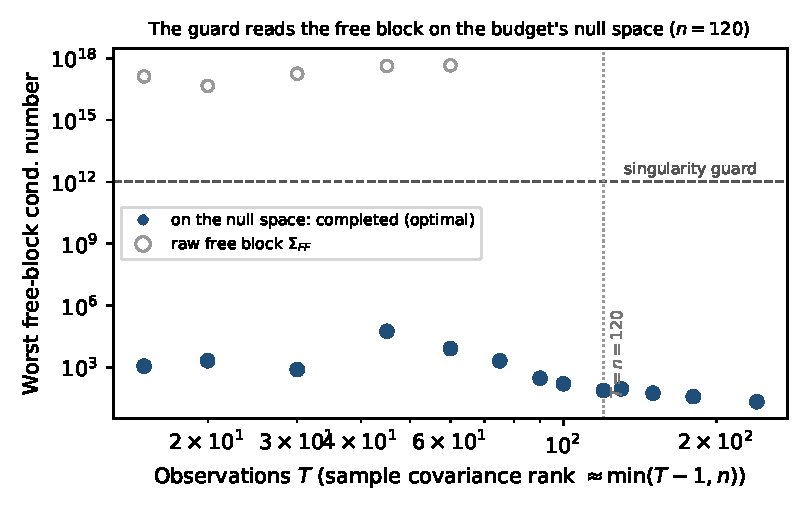
\includegraphics[width=0.5\textwidth]{degeneracy.pdf}
\caption{A rank-deficiency sweep at $n = 120$, the long-only covariance estimated from
$T$ observations. Grey rings are the worst condition number of the raw free block
$\Sig_{\F\F}$ over a trace; blue circles that of $Z\trans\Sig_{\F\F}Z$, the block on the
budget's null space, which is what the guard (dashed, $10^{12}$) reads. Below $T = 75$
the raw block is singular ($\sim\!10^{17}$) while the reduced block stays below
$6\times10^{4}$, so every trace completes, and every completed frontier matches a
reference QP to $3\times10^{-13}$. Release~2.3.3 declined the five windows with
$T \le 60$.}
\label{fig:degeneracy}
\end{figure}

\paragraph{Conditioning.}
To see the guard on its own we prescribe the spectrum,
$\Sig = Q \operatorname{diag}(\lambda) Q^\top$ with $60$ eigenvalues spread geometrically
from $1$ to $1/\kappa$, under a long-only budget, and certify each trace
(\target{validate-conditioning}). With a random orthogonal
$Q$ the free blocks see only part of the spectrum, their worst condition number stays at
$5.9\times10^{9}$ for $\kappa = 10^{16}$, and every trace completes with KKT residuals
below $2.5\times10^{-14}$. With $Q = I$ the free block inherits the full spread: traces
up to $\kappa = 10^{12}$ complete and are certified (residuals up to
$5.5\times10^{-12}$), and from $3\times10^{12}$ to $10^{14}$ every trace is declined at
the guard, so here its value decides the outcome. At $\kappa = 10^{16}$ the smallest
eigenvalues are zero to working precision; the trace completes again, in $10$ turning
points, and is certified ($3.9\times10^{-15}$). It and \pkg{OSQP} reach different weights,
up to $0.94$ apart, yet both meet the optimality conditions, so there the optimum is not
unique.

The reference QP is the less accurate of the two: OSQP leaves KKT residuals near
$10^{-9}$ and differs from the trace by up to $0.2$ in a weight in the diagonal family,
where the KKT conditions only weakly determine the weights along directions of tiny
variance. None of the $192$ reference solves failed.

\paragraph{Event ties.}
Ties are handled by the least-index rule of \S\ref{sec:bland}. Across four deliberately
degenerate families of $32$ instances each ($n$ up to $240$; \target{tie-degeneracy}),
a trace counts only if it is optimal: every turning point must pass the KKT certificate
of Table~\ref{tab:kkt} to $10^{-8}$, so a frontier that ends but is wrong is reported
as such. Exactly tied means give $31$ certified traces; the other instance ($n=60$) is
declined partway along the frontier, at a degenerate turning point whose multipliers are
not unique. Exchangeable pairs (identical means and covariance rows) give $32$ certified
traces, and the tie-break never frees both members of a pair. A family of
$p\approx n/3$ group caps gives $32$, with up to $53$ rows active at once, and an
over-constrained family of $p=n$ overlapping caps, whose maximum-return vertex is
degenerate, gives $32$, with up to $240$ rows active at once. No trace is off the
frontier.

\paragraph{A correction.}
The first version of this paper, run with release~2.3.3, counted completions without
certifying them, and reported that the tied-means and exchangeable families all
complete. They did complete, but none is on the efficient frontier: certified, all $32$
tied-means and all $32$ exchangeable traces of 2.3.3 fail the certificate, and on the
tied-means family with $n\le120$ their objective exceeds that of an interior-point
solve by up to a factor of $26$. Both families share
the largest expected return between several assets, and 2.3.3 started such a frontier
at an arbitrary vertex of the tied face (\S\ref{sec:first}). The group-cap family was
right, and $30$ of the $32$ overlapping-cap traces were, the other two declined.

The tied-means and group-cap families, the full-rank windows of
Figure~\ref{fig:degeneracy} and both conditioning families satisfy the hypotheses of
Proposition~\ref{prop:termination} at every turning point, so for them termination is
the theorem. The others do not. In the exchangeable family all $1751$ tied turning
points satisfy the hypotheses. The overlapping-cap traces pass $2637$ ties, all with
dependent constraints, so for them only the weaker guarantees of \S\ref{sec:bland} hold.
The nine rank-deficient windows of Figure~\ref{fig:degeneracy} have a singular $\Sig$,
outside $\Sig\succ0$; all nine complete, the five with $T\le 60$ by solving on the
budget's null space. No trace used more than $1.5\%$ of the iteration cap
$100(n+p+1)$.
